% ============================================================
%  H. Holst, "The Problem of Time"
%  Fysisk Tidsskrift, 15. Aargang (1916-17), pp. 1-13.
%
%  ENGLISH TRANSLATION
%  Status: COMPLETE. Translated from transcription.tex (the Danish diplomatic
%  transcription, COMPLETE), never from the scan. Structure mirrors
%  transcription.tex 1:1: same paragraphing, same page markers % --- p. N ---
%  at the same joints, the one footnote at the same anchor, the Fig. 1 block
%  in the same place.
%
%  The third item in the Kroman relativity debate and the first reply to
%  Kroman's 1915 attack; ../relativitetsprincipet/note.md carries the whole
%  seven-item table.
%
%  RIGHTS: clear. Holst died in 1944; Danish copyright (life+70) expired at
%  the end of 2014.
%
% ------------------------------------------------------------
%  TRANSLATION CONVENTIONS -- this article
% ------------------------------------------------------------
%  * Standing method: ../../../TRANSLATION-PLAYBOOK.md; the cluster's shared
%    decisions are set out at greater length in
%    ../relativitetsprincipet/translation.tex.
%  * QUOTATION MARKS. Danish guillemets »...« -> English curly doubles.
%  * EMPHASIS. All 14 \emph{} runs carried over. NOTE that this compositor
%    treats Holst differently from Kroman: PROPER NAMES ARE NOT LETTERSPACED
%    here (Minkowski, Michelson, Maxwell, Einstein, Lorentz all plain), the
%    one exception being »Emil Cohn« on p. 7. The English follows exactly --
%    so, unlike the Kroman articles, the names in this piece carry no \emph{},
%    and that is not an oversight.
%  * "Bud" is Holst's term for whatever carries the signal -- a messenger,
%    of any speed up to the infinitely fast messenger of the thought
%    experiment. Rendered "messenger" throughout, and "Budsendelse" as
%    "dispatch" / "sending of a messenger"; the word has to stay neutral
%    between a light ray and an ideal infinitely fast carrier, which is the
%    whole point of his argument.
%  * "Samtidighedskonferere" (p. 11), a coinage, is rendered
%    "simultaneity-conferring" and kept in quotation marks as printed.
%  * THE MAXWELL FOOTNOTE, p. 7, quotes »Matter and Motion« IN DANISH. What
%    stands here is therefore a rendering back into English of Holst's Danish,
%    NOT Maxwell's own sentence, and it is marked as such in a comment at the
%    note. A reader who wants Maxwell's wording must go to Matter and Motion.
%  * DECIMAL AND CASE FRACTIONS as in the Danish; thin-spaced thousands kept.
%  * THE FIGURE, printed p. 8, is the transcription's TikZ redrawing copied
%    verbatim. Its lettering (L, R, S, v, "Fig. 1.") is language-independent
%    and is untouched; the long comment recording what was measured and what
%    was regularised lives in transcription.tex and is not duplicated here.
%  * PRINTER'S DEFECTS. p. 5's stray comma after a full stop is reproducible
%    and is reproduced; p. 11's doubled e in »Atomeeksplosionerne« is
%    orthographic and is only noted.
%
%  BUILD: pdflatex (libertinus + libertinust1math), like the Danish.
% ============================================================

\documentclass[12pt,a4paper]{article}
\usepackage[utf8]{inputenc}
\usepackage[T1]{fontenc}
\usepackage{libertinus}
\usepackage{libertinust1math}
\usepackage{textalpha}
\usepackage{amsmath}
\usepackage{tikz}        % for the redrawn Fizeau diagram, printed p. 8
\usetikzlibrary{arrows.meta}

% FOOTNOTES. One only, on p. 7, marked *) in the printing.
\renewcommand{\thefootnote}{*)}
\usepackage[english]{babel}
\usepackage{enumitem}
\usepackage[protrusion=true,expansion=true]{microtype}
\usepackage{setspace}
\usepackage[margin=1.2in]{geometry}
\usepackage{fancyhdr}
\setlength{\headheight}{15pt}
\usepackage{hyperref}

\hypersetup{
  pdftitle={The Problem of Time},
  pdfauthor={Helge Holst},
  hidelinks
}

\pagestyle{fancy}
\fancyhf{}
\fancyhead[LE,RO]{\thepage}
\fancyhead[RE]{\textit{The Problem of Time}}
\fancyhead[LO]{\textit{H. Holst}}

\setstretch{1.3}

\title{\textbf{``The Problem of Time''}}
\author{H.\ Holst}
\date{\textit{Fysisk Tidsskrift} 15 (1916--17), pp.~1--13\\[2pt]
\small Translated from the Danish}

\begin{document}
\maketitle

% --- p. 1 ---
% The title block stands in the preamble via \maketitle. Signature lines and
% running heads are printer's furniture and are omitted, as in the Danish.
In his article ``Relativitetsprincipet'', pp.~1---30 in the previous volume of
``Fysisk Tidsskrift'', Professor Kroman passes an unconditional sentence of
condemnation upon Einstein's so-called theory of relativity, which he
characterises as ``a decidedly self-contradictory and therefore impossible
view''. Presumably many physicists who in and for themselves concur in this
judgement will nevertheless be inclined to use the Einsteinian system of
formulae, on the consideration that it may be an approximate expression for
something correct and possibly lead to new discoveries, even if it is derived
from an incorrect conception. Whether the danger there is in working with
formulae whose real meaning is not understood can be outweighed by the
advantages the formulae offer can presumably be known only by the fruits; but
the danger is undoubtedly diminished by the fact that one can take refuge in
the Lorentzian interpretation of the phenomena. Little satisfactory as this
may seem, it may nevertheless be a good makeshift so long as the
contradictions which have occasioned the appearance of Einstein's theory have
not been got out of the world in some other way.

However the journal's readers may now view these things, I believe that the
attack which has been made from the Einsteinian side upon our concepts of time
may make it desirable that the problem of time should be taken up for closer
consideration with a view to Einstein's theory. In what follows an attempt in
this direction shall be made. It cannot be avoided that one thing and another
which has already been said in Prof.\ Kroman's article is thereby repeated;
but that article nevertheless hardly makes superfluous an exposition which
aims more directly at throwing light upon our concepts of time.

% --- p. 2 ---
% The two letterspaced runs below are the article's programme; the numerals
% 1) and 2) that introduce them are NOT spaced.
Under the domain of the problem of time there belong two essentially different
kinds of task, namely 1)~\emph{the ordering of points of time in temporal
sequence} and 2)~\emph{the measurement of lengths of time in units of time};
they will here in the main be treated each by itself.

As regards the ordering of points of time, the matter is to determine a point
of time under consideration as past, simultaneous or subsequent in relation to
one or more others. One has in this connection generally proceeded on the
assumption that before, now and after were ``qualities in our consciousness'',
fundamental concepts in our view of the world, fundamental forms of
apprehension, or whatever one may care to call it, and that it was neither
required nor possible to explain their meaning or to define them by something
still more fundamental.

After the appearance of the theory of relativity it is, however, emphasised as
Einstein's merit that he has perceived the necessity of giving a definite
definition of simultaneity between events at different places in space, and
has moreover made the remarkable discovery that it was impossible to make such
a definition unambiguous. The truth would rather seem to be that the concept
of simultaneity which follows from the nature of our consciousness in reality
entered earlier, without definition, in the right way into the physicists'
trains of thought, while Einstein's definition has created confusion, because
it has brought it about that limitations in our physical means of determining
simultaneity have been exalted into something fundamentally essential for our
knowledge. But since doubt has been aroused in this matter, it may be useful
to make quite clear to oneself what is the real content of the concept of
simultaneity (for events at different places) hitherto used without closer
explanation, and this is at bottom not difficult.

% The place-letters A and B are ITALIC throughout, but the compound
% »A-Klokkeslet« sets its A in ROMAN in the printing. Set as printed, here
% as in the Danish: A-clock-time with an upright A.
Let us think of two places $A$ and $B$ --- which may be in motion or at rest
in relation to each other. From $A$ there is sent out, at a point of time to
which we may give the designation $t_{1}$, a messenger to $B$, where it
arrives at a for the present unknown point of time with the designation $t$
(in A-clock-time). The messenger is sent from $B$ straight back to $A$ and
arrives there at the point of time $t_{2}$. We shall then for the present
establish that $t$ lies between $t_{1}$ and $t_{2}$. The shorter this interval
of time is, the greater is the average velocity with which the messenger has
traversed the outward and the return path, provided these are straight lines.
Properly, certain reservations should here be made (for an oscillating motion
of $B$); but they lose their significance when the interval of time
$t_{1}\,t_{2}$ becomes sufficient\-%
% --- p. 3 ---
ly small. If we now think of the messenger's velocity as increasing
indefinitely, while the interval $t_{1}\,t_{2}$ decreases towards zero, or in
other words that the two events, the messenger's dispatch and its return,
approach indefinitely to simultaneity, the point of time $t$ for the
messenger's arrival at $B$ will also approach indefinitely to simultaneity
with $t_{1}$ as well as with $t_{2}$.

One may give what has here been developed the following more definitional
expression: two events at the places $A$ and $B$ are simultaneous when a
dispatch of a messenger, \emph{however fast the messengers used may be}, can
be arranged in such a way that a messenger from $A$ arrives at $B$ and departs
again from there simultaneously with the ``$B$-event'', while the point of
time for the ``$A$-event'' lies between the points of time for the messenger's
departure from $A$ and its return.

One might ask whether by this definition of simultaneity at two places full
reciprocity is attained, that is to say, whether an event at $B$ which has
been found to be simultaneous with an event at $A$ by a dispatch from the
last-named place would also be found simultaneous with it if the dispatch went
out from $B$; since one of the messenger's journeys did after all set out from
$B$ at the very moment the $B$-event took place, this cannot be doubtful. ---
We can also connect events at three or more places in space in time by letting
the messenger take the way from $A$ back to $A$ round by them all.

One might object that we are not able to send any messenger with infinitely
great velocity, or even with a velocity so great that the interval of time
$t_{1}\,t_{2}$ always becomes of vanishing magnitude in relation to our usual
measures of time: our fastest messenger, the light ray, takes years to
traverse the way between the earth and the nearest fixed star. This objection,
however, does not touch the core of the matter at all. What is in question
here is not at all how exactly we can carry out a determination of
simultaneity with the means at our disposal, but rather what lies in the
concept of simultaneity. With regard to this there has not previously been any
disagreement between physicists and other people. When a man, in order to
determine the point of time of an event, looks at a clock and establishes that
it happened at such and such an hour by the clock's indication, that is to
say, that it occurred simultaneously with the hand's passage over a definite
mark on the dial, he thereby proceeds, consciously or unconsciously, on the
assumption that light rays, nerve currents and the like have been messengers
so fast, the ways they had to
% --- p. 4 ---
traverse so short, and therefore the whole time for the dispatch so slight,
that the deviation from the ideal simultaneity determined by infinitely fast
messengers is without significance for his purpose; (Einstein too must
presumably, when he speaks without preceding definition of simultaneity
between positions of clock hands at $A$ and events in ``$A$'s immediate
surroundings'', proceed on the same presupposition). And when the physicist
compared points of time under conditions where the time for the dispatch could
not be regarded as vanishing, he took this time into the reckoning as well and
as exactly as was possible and necessary for the purpose, and thereby
proceeded on a concept of simultaneity agreeing with the definition on p.~3.

% The only inline case fraction with a built-up numerator on the page; set
% \tfrac, as the printing sets it small and on the line of text.
The definition of simultaneity between points of time at different places
without relative motion which Einstein set up in 1905 did not in and for
itself stand in conflict of principle with the aforementioned definition
either, since the latter would give the same result
$t = \tfrac{1}{2}(t_{1} + t_{2})$, provided the presupposition made by
Einstein, that light took an equally long time on the outward and the return
path, was correct. But since his dogma of the constancy of the velocity of
light led to results which stood in conflict with the ordinary concept of
simultaneity, this had, like other refractory concepts, to give way to the
dogma, and then there was proclaimed --- by Minkowski and others --- ``a
complete revolution of our ideas of space and time'' as an epoch-making result
of exact physical measurement and exact mathematical thinking.

It was immediately evident that a velocity greater than that of light would be
fateful for the whole structure of thought, especially for its paradoxes of
simultaneity. It was doubtless felt that the circumstance that the velocity of
light is the greatest velocity hitherto known was far too weak a defence for a
theory which went straight at our fundamental concepts. One believed, however,
that one could go a step further and declare the velocity of light to be the
greatest physically possible velocity; in support of this it is adduced that a
moving body's energy becomes infinite at a velocity like that of light; but
even if this could be regarded as proved, it is not thereby excluded that a
velocity of propagation (gravitation's?) might exceed that of light. Real
significance for our conception of time this question has not, however; for
even if the velocity of light occupies a special position in the physical
respect, it does not occupy a special position for thought. One might say that
we know very well a far greater velocity, namely that with which
% --- p. 5 ---
thought is able to fly to the outermost limits of the Milky Way in a vanishing
moment. Since one or another might have misgivings about thus placing side by
side a mental and a physical velocity, it will perhaps nevertheless be better
to keep to the mode of expression that we can think of velocities a thousand,
a hundred thousand and any number whatever of times as great as that of light,
and that we are entitled to consider Einstein's theory, like everything else
in the world, in the light of such a thought-experiment.

% PRINTER'S DEFECT, p. 5: a stray comma stands after the full stop of
% »fysiske Aarsag.« -- »Aarsag. , Hvis to Ure er«. Reproduced here.
This test in thought is, however, not the only one that can be applied. We can
also take our starting point in the determination of simultaneity by clocks
carried along, which plays so great a part here on earth. In principle it is
quite independent of the velocity of light, and it has as its only
presupposition that every change in the course of some process or other, for
example a change in a clock's rate, must have its definite and sufficient
physical cause. , If two clocks are absolutely alike in build, and are at a
definite place set alike to begin with, they will, subjected to the same
physical conditions, constantly keep together. This agreement will not cease
because the one clock is moved to another place, in so far as it is not
thereby exposed to other physical influences (that is to say, influences from
the material world about it) than those it was subjected to at the place of
departure. If we now let one of the two clocks brought into agreement at $A$
go along with the messenger to $B$ under the method of dispatch spoken of
earlier, the messenger would --- on the presupposition named --- so to speak
transport the place $A$'s time-indications with it and make it possible at $B$
to set clocks accordingly; as is seen by going to the limit (the infinitely
great velocity), one would thereby give simultaneous points of time (by the
earlier definition) the same designation at $A$ and $B$; there is, in other
words, no discrepancy between the two methods of determining simultaneity.

% Case fractions: the printing sets a superior 1, a solidus and an inferior
% 1000, all in roman. As in ../relativitetsprincipet.
In radium we have perhaps an ideal carried clock, since its degradation seems
independent of all external influences; if this really is the case, two pieces
of radium, of which the one remained at the place $A$ while the other went
from $A$ on a journey out into the world, should constantly keep together in
degradation, so that when at a certain point of time after the separation
$^{1}\!/_{1000}$ of the one's atoms had exploded, there would simultaneously
have exploded $^{1}\!/_{1000}$ of the other's. However this may stand, we can
at all events think of clocks which were com\-%
% --- p. 6 ---
pletely independent of, protected against, or compensated for all influence of
changes in temperature, pressure, gravitation, magnetic and electric fields or
other physical conditions at the point of space where the clock happened at
the moment to be. Besides these influences, dependent on the states in the
points passed, there might be conceived a physical influence due to the very
motion of the clock through a medium, the ether. Such an ``ether wind'' of
unknown magnitude and direction would introduce a hypothetical element into
our determinations of simultaneity; but even if we could not get beyond the
uncertainty thereby called forth, this would not compel us to alter our
ordinary conception of time and space. But if one, like Einstein, does not
assume any such ether wind or a corresponding physical influence, an alteration
of the clock's rate merely by the motion would, as Prof.\ Kroman emphasises,
be ``a causeless phenomenon'' --- a physical effect without a physical cause.
It seems to me that this is quite decisive for the question whether the real
alterations in clocks' synchronism (or twins' equality of age!) which are
assumed by Einstein's adherents to result from the one clock's (the one
person's) journey in space are acceptable from a physical standpoint. Just as
little as the clocks' rate can the measuring rods' length be altered by the
motion; but when one, by carrying a measuring rod that has been compared in
France with the right standard metre ``on board'' other moved systems $B$,
$C$ . . ., makes it possible in these to produce right metres, Einstein's
% The suspension above is printed as three widely spaced full stops, not as an
% ellipsis sort; set as printed, here as in the Danish.
ingenious method for comparing measuring rods (the setting of marks during the
passage at supposedly simultaneous points of time) becomes superfluous. When a
clock is transferred as well, the dispute about the points of time also falls
away, since indeed the transferred clock's indications, as well as the
transferred measuring rod's, must be decisive, and the discrepancies with them
show quite plainly that there is something wrong in the measurements which
give divergent results, or rather in the Einsteinian presuppositions on which
they rest.

% »for Sagen: men« -- a COLON, not a semicolon, in the printing. Kept.
Neither the transfer of, nor the Einsteinian experiments with, clocks and
measuring rods can be carried out in practice under conditions where the
results can reach such exactness that they are of significance for the matter:
but the placing side by side of the thought-experiments with the infinitely
fast dispatch and the transfer of clocks on the one hand, and the Einsteinian
transactions on the other, may contribute to throwing light on the new
theory's relation to the natural conception of time. That relation
% --- p. 7 ---
seems to me to signify not a \emph{revolution} of this conception, but a
\emph{destruction} of it. If we shake it, then we shake the very foundation
upon which we are to build up physics' picture of the world; we are carried
out into a condition where a mathematical system may indeed be created, but
where the natural control fails, so that absurdities get free play provided
only they fit into the system.

We apprehend existence in the form of space and time. As regards time this
means that we seek to arrange all events in the whole world in a continuous
series of groups whose events are mutually simultaneous, but past or
subsequent in relation to other groups. Physics has, however --- for the
material phenomena --- not merely this purely historical task; it is also to
find laws which are general, that is to say, independent of the point of
time\footnote{``The difference between one event and another ought not to
depend upon a difference in time alone'', says Maxwell in ``Matter and
Motion''.} and of the place (as such), and by which one may derive the events
% THE NOTE QUOTES MAXWELL IN DANISH. What stands above is a rendering back
% into English of Holst's Danish, NOT Maxwell's own sentence; a reader who
% wants Maxwell's wording must go to Matter and Motion. Holst's Danish is
% kept verbatim in transcription.tex.
in any group from those in any group past in relation to it.

There had now, however (through Michelson's experiment), been demonstrated an
apparently inexplicable distortion in the picture of the world which the
physicists had shaped, in that the earth might seem to be standing still with
respect to the ether, thus either to stand still itself or to drag the whole
world-ether along with it in all its motions. In order to get over this
difficulty Einstein had recourse to the expedient of introducing a multiplicity
of world-pictures (as many as there are in the whole world systems of
particles with different translational motions), each burdened with its
individual distortion. Since this distortion was of quite the same kind in the
different world-pictures, which were all declared to be equally good, one got
\emph{uniformity} or symmetry as a surrogate for the abandoned \emph{unity};
and even if the individual world-pictures did not admit of being reconciled
with one another, it was nevertheless possible to convert the one into the
other by simple formulae; thus once more a surrogate: \emph{convertibility}
for \emph{agreement}. Considering that Einstein has thus abandoned the monism
which has hitherto always been aimed at in the conception of the material
world, and has gone over to a peculiar kind of ``polyism'', it sounds almost
like a bitter irony when \emph{Emil Cohn} in his little work ``Physikalisches
über Raum und Zeit'' asserts that by Einstein's
% --- p. 8 ---
theory greater unity has come into our picture of the world (``. . . unser
Weltbild wird einheitlicher''). Philosophically regarded, his doctrine is to
be rejected, because it destroys our conception of the world and puts many
mutually irreconcilable --- but by simple formulae connected --- truths in the
place of one. Physically regarded it becomes to be rejected as well, because
where one seeks physical causes it offers mathematical transformations
instead. We may say that the abandonment of the historical demand that all
events be arranged in a universally valid temporal sequence entails the
abandonment of the physical demand that causal connection be established
within the material world.

For the illustration of this side of the matter there shall here be considered
the case, brought forward by Prof.\ Kroman as well, concerning the velocity in
flowing water.

% ================================================================
% FIGURE, printed p. 8.  EDITORIAL REDRAWING IN TikZ -- NOT A FACSIMILE.
% Copied verbatim from transcription.tex, whose comment records what was
% measured off the 600 dpi page image and what was regularised. The block's
% lettering (L, R, S, v) is upright bold sans in the printing, not the italic
% the running text uses for the same letters, and is language-independent;
% nothing here is translated.
% ================================================================
\begin{center}
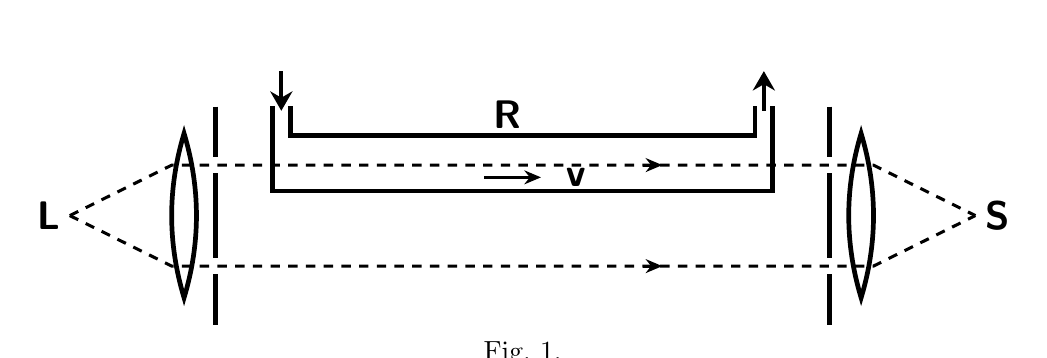
\begin{tikzpicture}[x=0.006cm,y=0.006cm,
    apparatus/.style={line width=1.7pt},
    stopline/.style={line width=2pt},
    ray/.style={line width=1.1pt,dash pattern=on 3.4pt off 3pt},
    head/.style={line width=1.1pt,-{Stealth[length=6pt,width=5pt]}},
    water/.style={line width=1.4pt,-{Stealth[length=7pt,width=8pt]}},
    letter/.style={font=\Large\sffamily\bfseries}]

  % --- the water tube R: a channel open at both ends ---
  \draw[apparatus] (-492,232) -- (-492,169) -- (492,169) -- (492,232);
  \draw[apparatus] (-530,232) -- (-530, 52) -- (530, 52) -- (530,232);

  % --- water in at the left neck, out at the right ---
  \draw[water] (-511,306) -- (-511,222);
  \draw[water] ( 511,222) -- ( 511,306);

  % --- the two lenses, pointed at top and bottom as the block draws them ---
  \draw[apparatus] (-717,-174) .. controls (-752,-58) and (-752,58) .. (-717,174)
                               .. controls (-682, 58) and (-682,-58) .. cycle;
  \draw[apparatus] ( 717,-174) .. controls ( 682,-58) and ( 682,58) .. ( 717,174)
                               .. controls ( 752, 58) and ( 752,-58) .. cycle;

  % --- the two stops, broken where the rays cross ---
  \draw[stopline] (-650, 231) -- (-650, 124);
  \draw[stopline] (-650,  90) -- (-650, -90);
  \draw[stopline] (-650,-124) -- (-650,-231);
  \draw[stopline] ( 650, 231) -- ( 650, 124);
  \draw[stopline] ( 650,  90) -- ( 650, -90);
  \draw[stopline] ( 650,-124) -- ( 650,-231);

  % --- the two ray bundles: through the tube, and below it through the air ---
  \draw[ray] (-959,0) -- (-743, 107) -- (743, 107) -- (959,0);
  \draw[ray] (-959,0) -- (-743,-107) -- (743,-107) -- (959,0);
  \draw[head] (255, 107) -- (296, 107);
  \draw[head] (255,-107) -- (296,-107);

  % --- direction of flow ---
  \draw[head,line width=1.2pt] (-81,81) -- (39,81);

  % --- lettering ---
  \node[letter,anchor=east] at (-959,  0) {L};
  \node[letter,anchor=west] at ( 959,  0) {S};
  \node[letter]             at ( -33,214) {R};
  \node[letter]             at ( 113, 80) {v};

  % --- the printed caption ---
  \node[anchor=north,inner sep=2pt] at (0,-253) {Fig.~1.};
\end{tikzpicture}
\end{center}

In Fig.~1 Fizeau's experiment is indicated in simplified form. From the light
source $L$ a bundle of light rays is sent through the air, another through the
water-filled tube $R$ to $S$, where interference fringes are formed, and these
are displaced when the water is made to flow through the tube with the
velocity $v$ in the direction of the arrow. As is well known one finds a
displacement corresponding to this, that the light's velocity in the stretch
of tube is altered by the flow from $\dfrac{c}{n}$ to
$h = \dfrac{c}{n} + \dfrac{n^{2}-1}{n^{2}}\,v$ in relation to the tube wall,
and thus to $h' = \dfrac{c}{n} - \dfrac{v}{n^{2}}$ in relation to the mass of
water. There then arises the question why the light gets precisely this
velocity, instead of, for example, preserving an unaltered velocity either in
relation to the water or in relation to the tube wall.

The physicist means by this question that he wants a closer account of the
matter. He wants clarity about wherein the physical processes which take place
in the tube when the water flows differ from those which take place when it is
at rest. He will next seek either
% --- p. 9 ---
to bring a previously known and more general rule to bear on the case in hand,
or to set up a new plausible theory which can be applied both to this case and
under other conditions. But already to penetrate into the nature of the
processes, or merely to have one's eye opened to certain possibilities in this
respect, is a real advance on the physicist's road of work. One might, for
example, make the quite crude assumption that the light passes alternately
through the atoms of the substance (or condensed ether-spheres about them)
with a certain velocity $c_{1}$, and through the free space between them with
the velocity $c$. In the flow the atoms are carried along with the velocity
$v$, and it might then be conjectured that the light preserved its velocity in
the empty spaces as well as inside the atoms (in relation to these); at a
certain ratio between the ``atomic diameters'' and the ``free paths'' one
would get the result the experiment gives. But it might also be thought that
the velocity of propagation itself inside the atoms was altered to $c'_{1}$,
because the light met the atoms with another (relative) velocity. Or one might
assume that the light can slip through the interspaces of the atoms, but that
its velocity at rest is reduced, by the action of the atoms' ``force fields'',
to $\dfrac{1}{n}$ of the velocity in free space; the atoms' motion (in
relation to the ether?) would then alter this influence, whereby the light can
get another velocity in relation to the tube wall as well as in relation to
the water. Or it might be that the velocity with which the front of a wave
advanced was not altered by the water's motion, but that the electrons in the
mass of water acted upon the phase of the light motion in such a way that
``the phase's velocity'', which is of course determinative for the
interference, was altered; $h$ and $h'$ would then denote the phase's
velocity. (Which of these or of other possible assumptions is the right one
plays no part in this connection.)

The Einsteinian treatment of the question is, however, of quite another kind.
By the application of his transformation formulae one finds that a being which
goes along in the water's translation should, by any measurements it might
make, come to the result that the light motion inside the water has, in
relation to this, not the velocity
$\dfrac{c}{n} - \dfrac{v}{n^{2}}$ but rather the velocity $\dfrac{c}{n}$,
quite as we find it when the water stands still for us. Even apart from the
fact that this is incomprehensible, it cannot
% --- p. 10 ---
be regarded as an explanation. What \emph{I} need is to get coherence into
\emph{my} picture of the world; if I cannot get it, it is but a poor
consolation that another calls right what I call wrong, especially when I know
at the same time that he finds wrong what I find right, so that I should gain
nothing by going over to his view of things.

One might say to this that even if Einstein's theory gives no proper
explanation of the matter, one could nevertheless in the case considered, by
going the opposite way --- that is to say, by starting from the simple
assumption that for an observer carried along with it the velocity of light in
the water is always $\dfrac{c}{n}$, and using Einstein's transformation
formulae --- calculate a correct expression for the drag-coefficient which
presents itself for observers not carried along with it. This is doubtless
true enough; but it is not the question of the use which Einstein's system of
formulae may possibly be of that is to be discussed here. There might however,
particularly on the occasion of Prof.\ Kroman's remark on p.~24, be reason for
this special case to emphasise that the drag-coefficient
$\dfrac{n^{2}-1}{n^{2}}$ can also be derived without the help of the
Einsteinian formulae, for example by setting up the condition that light which
is led forward through a stretch of standing water and back through a stretch
of air, and light which traverses the same way in the opposite direction,
shall get no demonstrable interference-producing path difference from the
motion of the experimental apparatus through the ether (with the earth); since
now Einstein's formulae are constructed precisely so that the ``ether wind's''
influence shall by them disappear from the calculations as it does from the
experiments, it was presumably really given in advance that in the case
considered they would give the same result as one can get by directly writing
down the conditions for the ether wind's having no influence.

As we now pass over to the other part of the domain of the problem of time,
namely the measurement of lengths of time, we ought to notice that nowhere in
what has been said above about the determination of simultaneity has any use
been made of the concept of uniform motion. Of the clocks (p.~5) it was merely
presupposed that they, when they were quite alike and were exposed to quite
the same physical influences, would constantly keep together; whether they go
uniformly is quite another matter. This notwithstanding, one can by means of
the clocks compare lengths of time at different \emph{places}, in that two
lengths of time which lie between two sets of two-by-two
% --- p. 11 ---
simultaneous points of time for events at two places are set as equally long.
But we cannot, in the nature of the case, get any sure criterion that two
lengths of time which elapse at different \emph{times} are equally long. One
can only compare such lengths of time by ``simultaneity-conferring'' them with
a time-measurer which goes uniformly; but that this is the case must again be
established by comparison with another time-measurer, and so on.

% PRINTER'S DEFECT, p. 11: the Danish sets »Atomeeksplosionerne« with a
% doubled e. Orthographic and not reproducible in English; the transcription
% carries it.
One might get beyond this difficulty by keeping to a time-measurer of which
one must, on the basis of one's whole knowledge of the physical world, assume
that its rate does not alter in the course of time. The rotating earth is not
such a time-measurer, since we can see causes for its period of revolution
decreasing. Rather would one presumably acknowledge a measurement of time
based on the light motion, taking as an unalterable measure of time the time
light takes to traverse a definite length --- for example a length equal to
the diameter of an electron (disregarding the assumption of the latter's
alterability, or thinking of the closer circumstances as settled). Apparently
one might escape mixing lengths into the matter at all, by for example using
radium as time-measurer and setting the time in which $^{1}\!/_{1000}$ of a
piece of radium's atoms exploded as the measure of time; but since the atomic
explosions are only clock-strokes for a process running its course in space
and time in the interior of the substance, one does not thereby avoid having
to do with lengths. The questions of a constant measure of time, a constant
measure of length and a constant velocity stand in close mutual connection.

Even if there can be found in nature lengths, intervals of time and velocities
which cannot be assumed to be altered in the course of time by any of the
physical processes known to us, we cannot nevertheless exclude the possibility
that they are altered by some universal cause unknown to us, and in such a way
that we cannot check it at all. (The Lorentzian contractions from an ether
wind whose velocity and direction are unknown to us afford precisely an
example of uncheckable alterations.) Let us assume that the whole world, or at
all events that part of it which we know, were subjected to a continued
process of shrinkage whereby all lengths were diminished in the same ratio, so
that, for example, both the electrons' dimensions and the distances between
them had after a certain number of millions of years gone down to
$^{1}\!/_{10}$; then it would in the first place be impossible to establish
this by measurements of length
% --- p. 12 ---
with measuring rods which were themselves diminished in the same ratio. But
even if all velocities had remained unaltered, so that all processes now (on
account of the shorter distances) ran their course 10 times as fast, the
shrinkage could not be established by measurements of time either, since the
measure of time also (for example the time light takes to traverse an electron
diameter) had become 10 times as small, wherefore one would find the duration
of all processes expressed by the same numbers as before. Since all processes
in the brain and the nerves ran their course with tenfold velocity, one would
presumably have to assume that the same would hold of our whole course of
ideas, and that our time-sense, that is to say our immediate apprehension of
lengths of time, would undergo such a change that the ``shrinkage'' would not
make itself noticed in our consciousness at all. But even if we think of our
time-sense as remaining unaffected by the changes, so that we noticed that all
processes went on with a far greater speed than before, we could nevertheless
not decide whether this was due to the world's having shrunk, or to the
world-machinery's having really run wild --- or finally merely to a mental
change in our conception of time. Just as an increase of all velocities would
come to the same thing as a shrinkage of all lengths, a gradual slackening of
the world-machinery would act quite like an expansion of all lengths, and none
of these four phenomena would be demonstrable by physical measurements. By a
simultaneous shrinkage of all lengths and diminution of all velocities in the
same ratio, the duration of all processes would remain unaltered, so that even
with an intact time-sense we should not notice any change.

There is evidently in all this an abundance of ``relativity'', and the
considerations adduced may perhaps even make it doubtful whether any meaning
can be attached to concepts such as the absolute magnitude of a length, of an
interval of time and of a velocity. They seem afflicted with an indeterminacy
similar to that of the concept of absolute rest in an empty and infinite
space. With the concept of simultaneity the case is quite another. In order to
attach a definite meaning to two events at different places in space being
simultaneous, we do not need to ascribe an absolute magnitude to certain
lengths, intervals of time or velocities; it is sufficient that we can think
of alterations of them (pp.~2---3). One might object that we can indeed think
of a velocity 1000, 10\,000 or more times as great as, for example, that of
light, but
% --- p. 13 ---
that our thought can nevertheless never reach an infinite velocity, and
therefore not ``absolute'' simultaneity either; although this is in a way
right enough, it is nevertheless a sophism, not much better than the famous
one about Achilles and the tortoise. It will also be seen that the concepts
``absolute simultaneity'' and ``absolute magnitude'', as they are used here,
have nothing analogous about them at all; for in the first expression
``absolute'' means ``completely exact'', in the second ``without relation to
anything else of the same kind''.

The relativity which is inseparable from our concepts of time does not, like
the Einsteinian, come into conflict with our hitherto received conception of
time. It does not lead us into a mystical world where space has 4 dimensions.
It does not hinder us from remaining in the good old three-dimensional
world-space, where 3 and only 3 mutually perpendicular planes can be laid
through a point, where simultaneous events are simultaneous, where every
physical change has its physical cause, and where two railway trains which run
each to its own side with a velocity of 100 km an hour move apart from each
other with exactly the double velocity, whether we are passengers on the one
train or the other or stand outside and look on.
% The article ends here, in the middle of printed p. 13; the rest of the page
% is given to the opening of the next item, C. E. Walsøe, »Omkring
% Videnskabens Grænse«, which is no part of this text.

\end{document}
